\subsection{El model: Model Vista Controlador}\label{sec:mvc}

    \paragraph{}
    A l'hora de crear l’aplicació web, volíem crear-la mitjançant una estructura comprensible i eficient, on cada tecnologia realitzes el seu rol principal i deixés aquelles tasques per les quals no havia estat concebuda, a altres tecnologies.

    En el món del desenvolupament web, predomina una arquitectura de tres capes que emula el model vista controlador. Però, en què consisteix exactament aquest model? El model vista controlador, també conegut com a MVC\footfullcite{wiki:mvc}, és un patró d'arquitectura pensat per la implementació d'aplicacions, que disposen d’una interfície d'usuari.

    Com bé indica el nom, el model és compost principalment per tres elements. El Model, la Vista i el Controlador. A continuació, descrivim amb més profunditat el rol de cada un d’aquests components.

    El Model és el principal encarregat de gestionar i manipular les dades amb les quals treballa el sistema. El Model, també s’encarrega de crear la lògica i regles, sobre les quals l'aplicació funciona. D’aquesta forma, aquest component serà l’encarregat de gestionar les connexions amb les bases de dades, en cas que aquestes existeixin i crearà els blocs de dades a retornar, de forma que puguin ser compresos pel Controlador.

    La Vista o Vistes, representen les representacions visuals de la informació. En altres paraules, la interfície que l’usuari veurà i amb la qual podrà interactuar. Mitjançant les interaccions amb aquesta interfície d'usuari, l'usuari és capaç d’indicar a l’aplicació, quines són les accions que vol que realitzi.

    Finalment, el Controlador s'encerrega de recollir els diferents inputs enviats per l'usuari, validant-ne l'estat i comunicant-lo a la capa del Model, per obtenir les dades o recursos (entesos com a fitxers servits per la capa Model), demanats per l’usuari. En cas de necessitat, el Controlador també és l’encarregat de modificar la vista o l’estat d’una vista, per reflectir, en tot moment, l’estat actual de l’aplicació a la interfície d’usuari.

    La gràcia d'aquest model és que l'usuari només disposa d'accés i permisos d'in\-te\-rac\-ció a la capa de les vistes. Aquestes, comuniquen les accions realitzades per l'usuari al controlador, que a la vegada, s'encarrega de gestionar les comunicacions amb el model i quan aquest retorna dades, transmetre-les un altre cop cap a la vista.

    D'aquesta forma, l'ús de la capa model és completament transparent per l'usuari. La figura~\ref{fig:MVC}, mostra un exemple de com podria funcionar el model MVC en un cas ideal. En la nostra aplicació web, s'ha intentat seguir aquest model en la mesura que ha estat possible.

    \begin{figure}[h]
        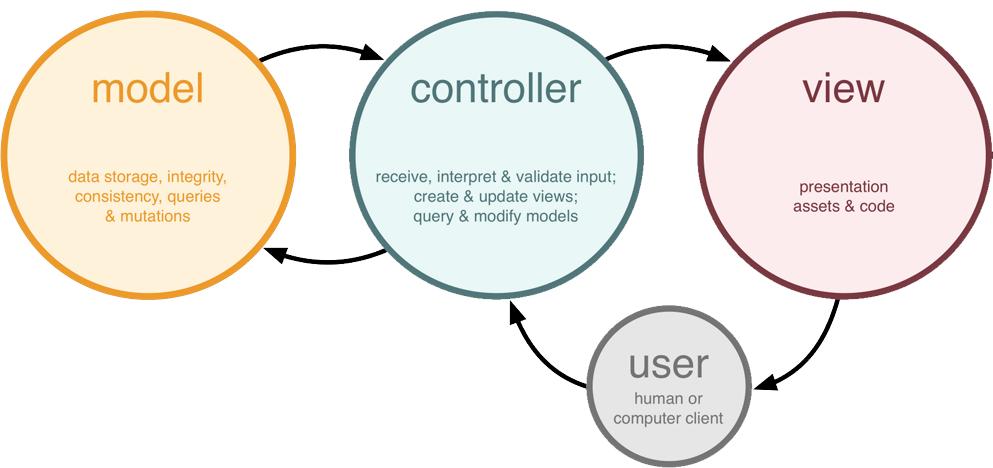
\includegraphics[width=\linewidth]{08/01_MVC}
        \centering
        \caption{Exemple de funcionament del model MVC.}\label{fig:MVC}
    \end{figure}

    Un últim aspecte important de cara a la terminologia d'aquesta secció, és entendre com relacionem cada una de les capes del patrò MVC, amb els diferents elements que conformen una aplicació web.

    Les pàgines web, s'acostumen a poder dividir en dos grans conceptes o elements principals: el front-end i el back-end.

    El front-end, fa referència a la capa de presentació o amb altres paraules, el navegador de l'usuari i per tant, aquest element serà associat a la capa Vista del model MVC.

    Per altra banda, el back-end és el component que acostuma a realitzar l'accés a les bases de dades i prepara la informació que ha de ser servida al front-end. Per tant, en el nostre cas, el back-end jugarà el paper de la capa Model, en la nostra aplicació web.

    Finalment, el paper del Controlador, sol ser representat en una aplicació web com la part del codi del client (navegador), que l'usuari no veu, ni interactua directament amb ella. En alguns sectors, aquesta part d'una pàgina web es coneix pel nom del `back-end del front-end'.

    La figura~\ref{fig:webElementsEmpty} mostra els tres elements descrits de les aplicacions web i el paper que jugaran, dins del model MVC, cada un d'ells. Durant els següents apartats d'aquesta secció de la memòria, anirem emplenant cada una de les caixes, amb les diferents tecnologies que seran utilitzades.

    \begin{figure}[h]
        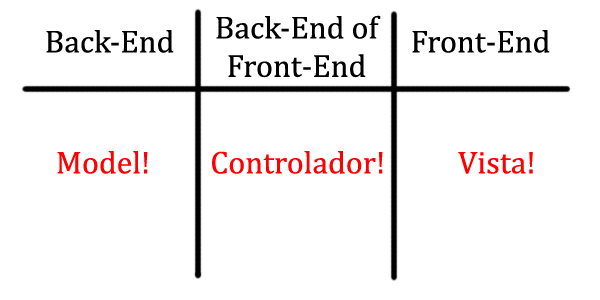
\includegraphics[scale=0.4]{08/02_webTechIni}
        \centering
        \caption{Elements de l'aplicació web i el patro MVC}\label{fig:webElementsEmpty}
    \end{figure}
